\section{Services}


\subsection{Authentication}

Services, by their nature, are accessible to remote clients. While the ultimate security policy for CLAS 12 GeV has not been addressed, the software group recognizes that some form of user authentication will be required. The authentication service will allow other services to ask whether or not a given user is authorized to receive the information he requested.

There are number of ways to implement such a service, including some powerful but platform specific solutions, such as the authentication suite provided by Microsoft .NET. Again, the loose coupling provide by a Service Oriented Architecture allows us to define the authentication interface �contract� even before we decide on an implementation, and it allows us to replace implementations to meet growing needs to address unforeseen security concerns.

So we plan to start with an authentication service that will accept a username and password and return an integer value for the user�s access level. (We may only ever need a no access/full access determination.) The first implementation of the service will just return a value indicating full access for all requests. That will allow other services to build in their authentication request. From there we will move to an actual implantation, perhaps one using an LDAP or MySQL server that stores username, passwords, and access levels. That may prove sufficient, but if not we can always to an even more secure authentication scheme without breaking the framework.


\subsection{Detector Geometry}

The Geometry service is an example of the Detector Data Service. This is the front-end of the CLAS12 geometry data, encapsulating data access and data management details from the service consumers. All the ClaRA algorithm services, including simulation, reconstruction, alignment, and etc. access the geometry service using standard service communication protocols, provided by the framework. Currently geometry information is stored in the mySQL database, but in the future we might consider changing the geometry data storage technology (for example XML) being fully transparent to the geometry service consumers.

\subsection{Event Display}

The single event display in the CLAS 12 GeV framework will be both a service consumer (a client) and a service provider.

Implementing the event display as a service consumer provides all the benefits discussed in the section of Service Oriented Architecture. Additionally it allows us to use the �thin client� model favored by modern software architects. Thin clients, sometimes called smart clients, split their application code between data models and processing, performed as much as possible in a different thread, process or CPU, and visualization. This shrinks the pure visualization code allowing it to be deployed remotely or updated frequently with incurring a huge download penalty. The most familiar and successful model is probably Google Earth. A thin client is downloaded an runs quickly, but complicated imagery processing is performed remotely. 

A service oriented architecture is one way to implement thin clients. As much as possible, without hampering performance, no visualization processing, such as acquiring detector geometry, is performed by a service and the thin client obtains the geometry by sending a request.

In the case of event display, the client will use a variety of services such as geometry, magnetic field, event streaming, file system access, run metadata, and analysis. It will also be a service provider through a display service. One service it will provide will include simple pictures of random on-line events so that remote users, for diagnostic purposes, can see pictures of recent events. Another more sophisticated service will be to answer a request for an image of a specific event viewed in a certain way, such as �zoomed in on region one in sector three.�


\begin{figure}[htbp] %  figure placement: here, top, bottom, or page
   \centering
   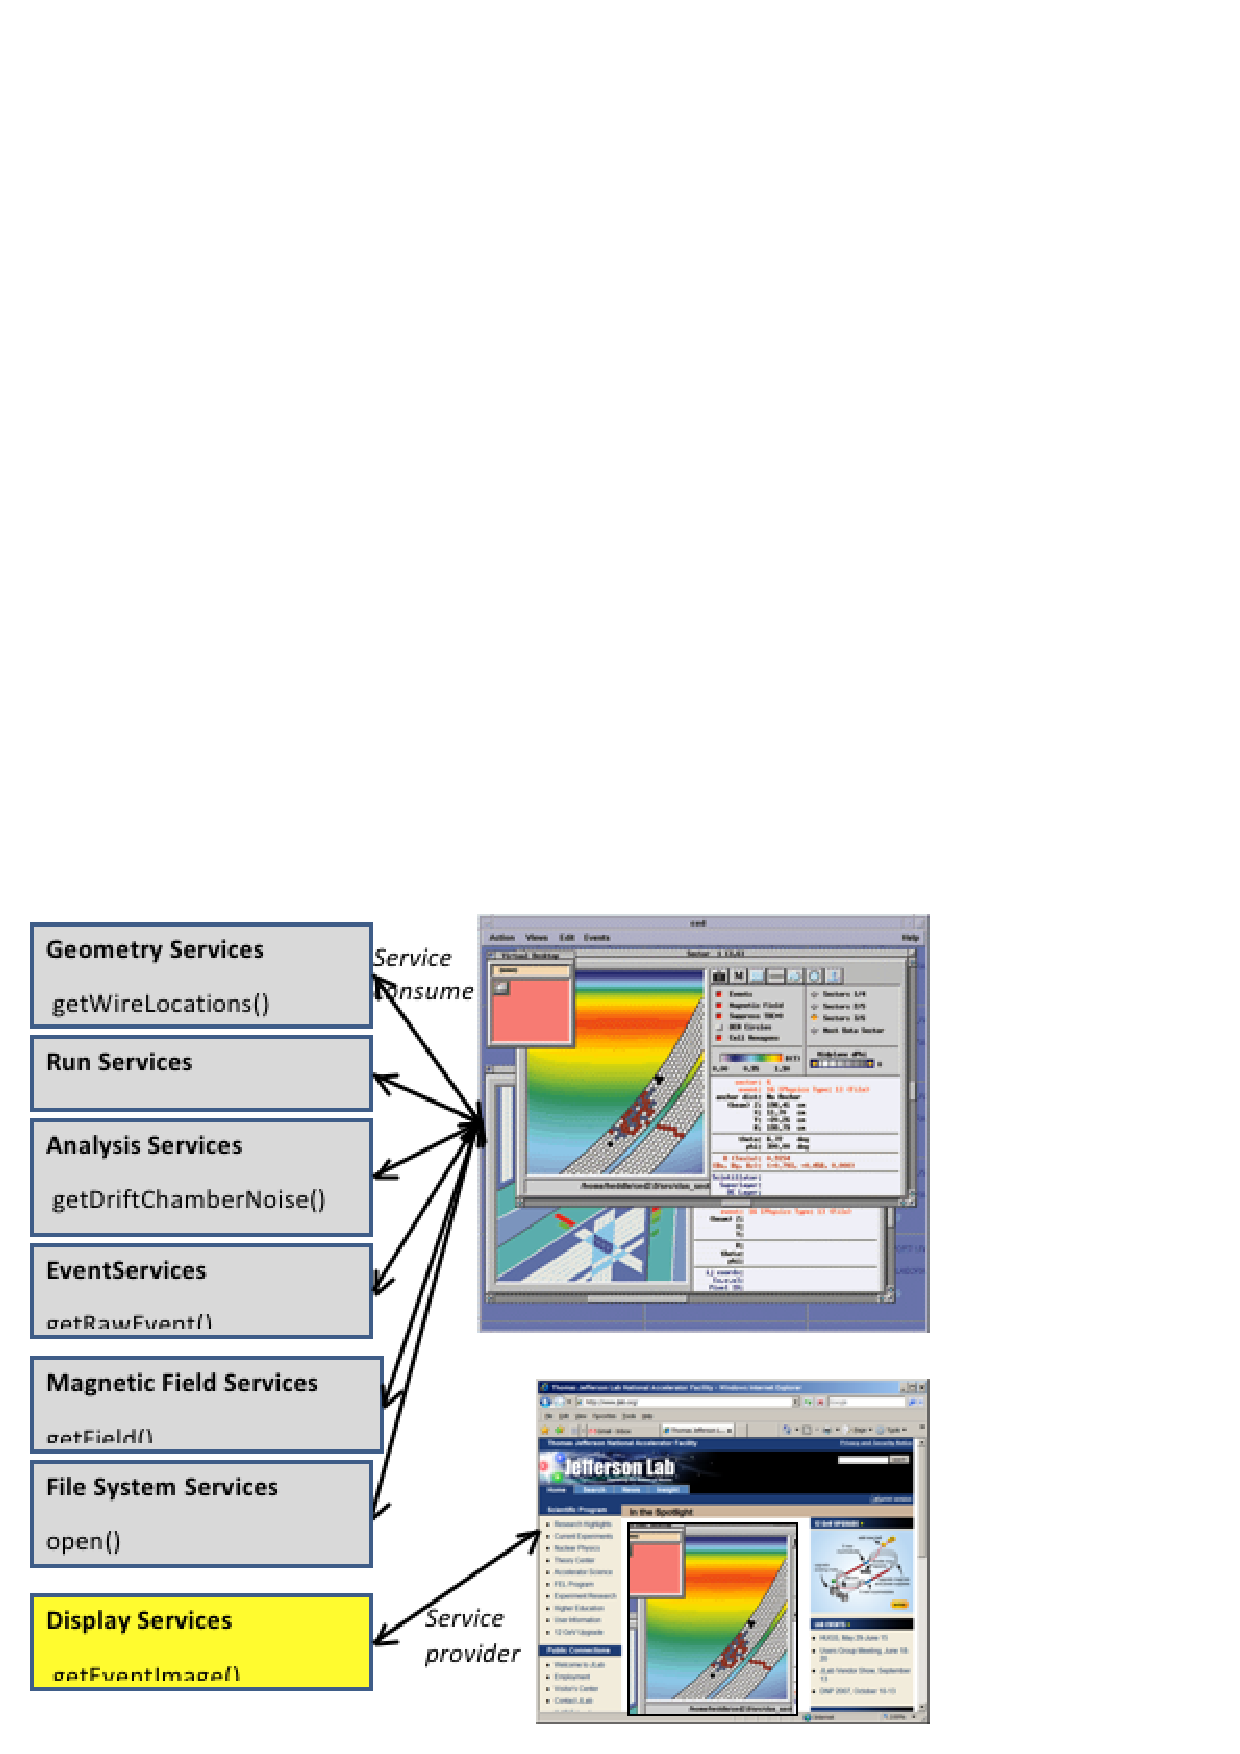
\includegraphics[width=5in]{Services/eventDisplay.png} 
   \caption{The event display will consume a number of CLAS 12 GeV services. It will also provide a display service.}
   \label{fig:eventDisplay}
\end{figure}

Another feature of the event display is that it will employ a plug-in architecture based on the reflection capabilities of the JAVA language. This will provide a simple yet powerful extendibility feature for users who would like to use the event display to visualize and debug their new analysis and simulation code. Reflection is a way that JAVA applications can examine all the classes in their path. The event display will look for all classes that inherit from a specific abstract base class. Once found, the application will create an object from that class and then provide a set of services for the object, such notifying it that a new event has arrived. 

In this scheme, not recompilation or even restart of the event display is required. The developer extending the event display creates the class, drops it into the path, and the class will be �plugged-in� to the application. If the plug-in proves of general use, it can be placed in the path of the shared event display (e.g., the run in the counting house) and all users will have access. On the flip side if it is found to be an undesirable or buggy feature, the class file can simply be deleted. All of this adding and removing of features will occur with no changes to the code or recompilation of the base event display. 


\subsection{Data and Algorithm Services}

In addition to our purpose to produce a Service Oriented Architecture based design, we have decided to separate data services from algorithm services. An algorithm service, in general, will accept and process an output data object from a data service and will then produce a new data object.
\subsubsection{Basic types of data services}
One of our main design choices is to separate data services dealing with the data objects that are resident on the disk from the data services which manipulate the data objects in the memory. An objective that we would like to achieve is to make algorithm services independent of the technology we use for data object persistency. This will allow replacing outdated persistency technology in the future without affecting user produced algorithm services. By separating persistent and transient data services we also hope to achieve higher level of optimization by targeting inherently different optimization criteria for persistent and transient data storages. For example, regarding the data objects on the disk one should invest more effort to optimize I/O performance, data size, avoid multiple I/O requests, etc. On the other hand, for the transient data in the memory we should achieve highly optimized execution performance, API and usage simplicity, etc.

We foresee three major categories of data objects:
�	Event data, such as raw data, simulated data, reconstructed data, etc.
�	Detector data, describing a detector apparatus in order to interpret the event data. Examples of the detector data are geometry data, calibration data, alignment data, slow control data, etc.
�	Statistical data (histograms, n-tuples, etc.)
Specific data services are provided for each of these data categories (see figure ~\ref{fig:service1}).


\begin{figure}[htbp] %  figure placement: here, top, bottom, or page
   \centering
   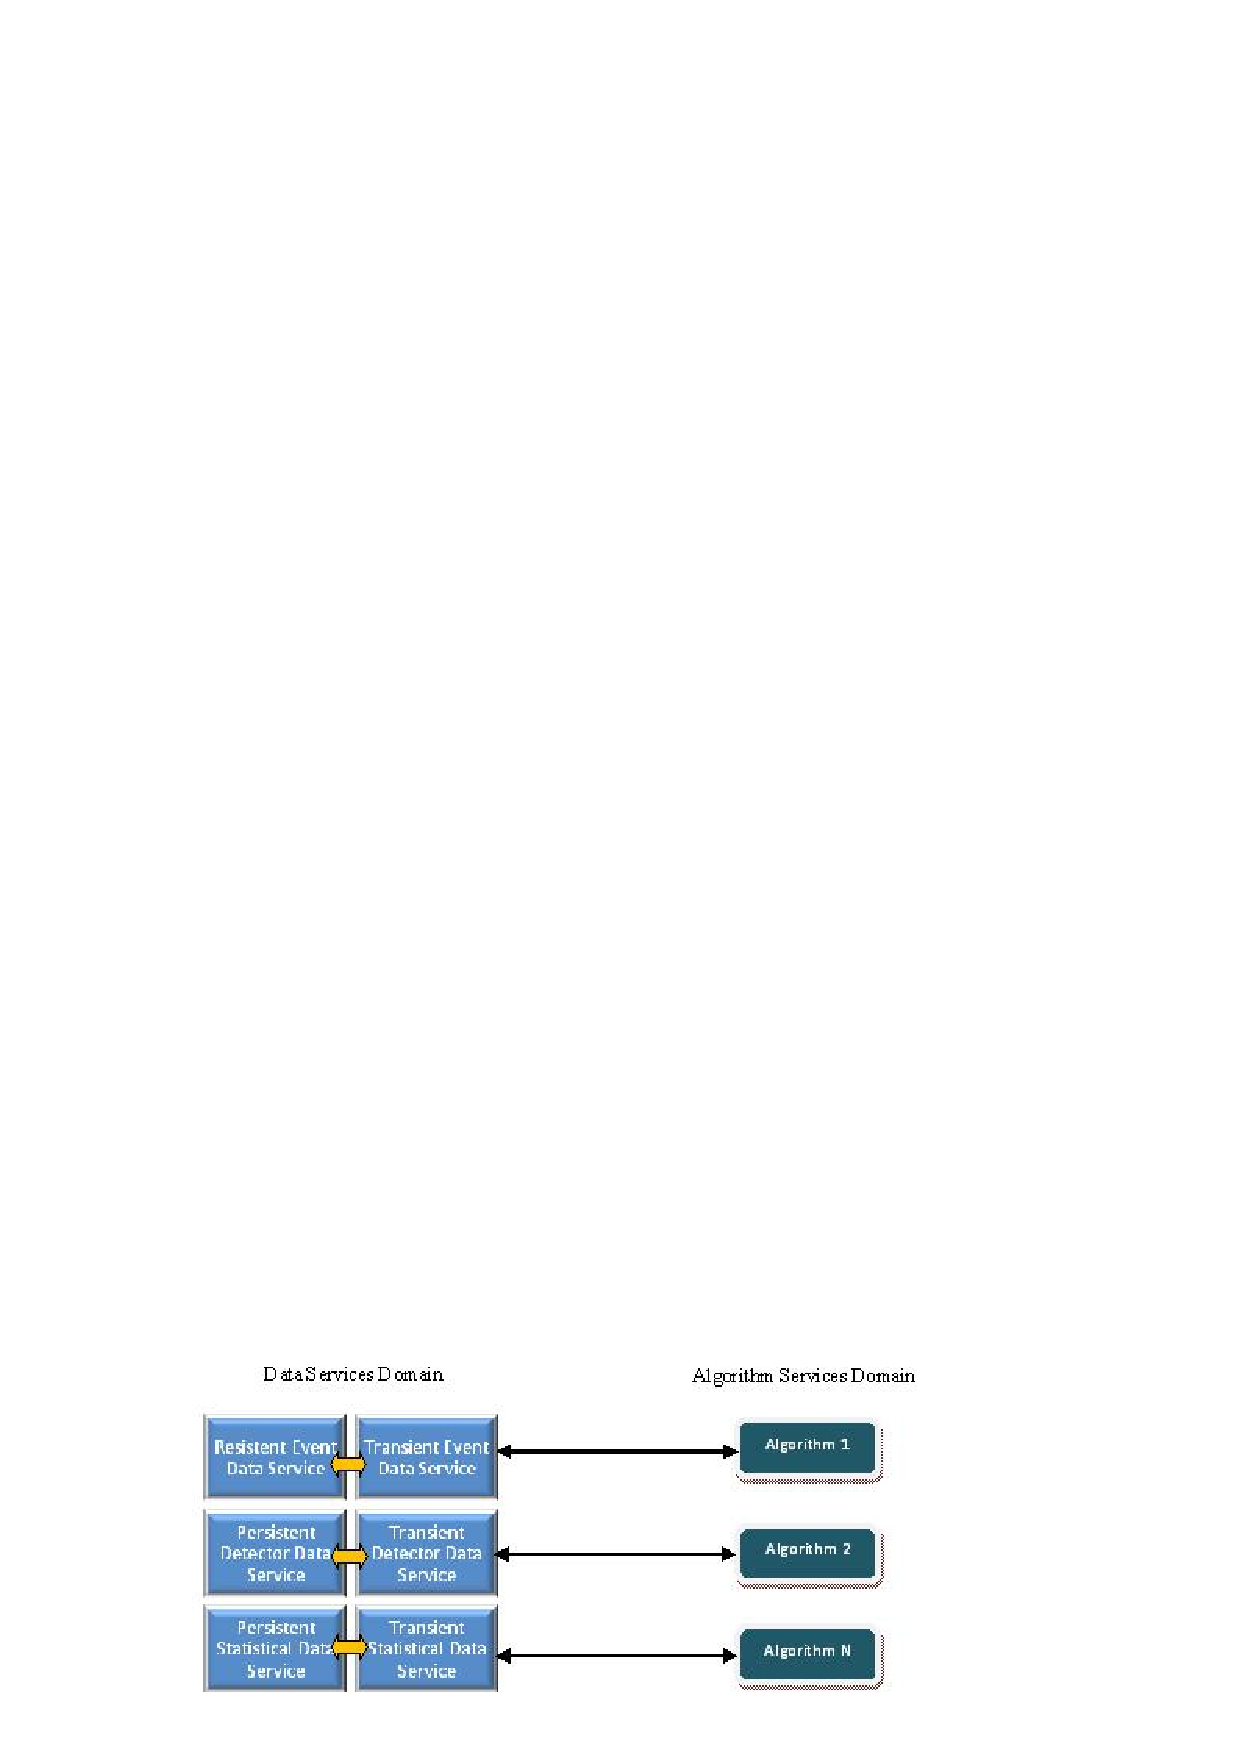
\includegraphics[width=6in]{Services/service1.JPG} 
   \caption{Different data services of ClaRA framework. Algorithm services deal with transient data services only.}
   \label{fig:service1}
\end{figure}
\subsection{Calibration Services}